\documentclass{beamer}
\ifxetex
 \usepackage{fontspec}
\else
 \usepackage[T1]{fontenc}
 \usepackage[utf8]{inputenc}
 \usepackage{lmodern}
\fi
\usepackage{amsmath, pdfpages, pdflscape, lscape, color, listings, hyperref, amssymb,graphicx,textcomp,varioref,afterpage,subcaption, float,color} 


% \makeatletter
% \def\input@path{{/home/simen/Dropbox/phd/presentations/presentations/neuronify}}
% %or: \def\input@path{{/path/to/folder}{/path/to/other/folder}}
% \makeatother

\title{Neuronify: a new tool for creating simple neural networks}
\author{Simen Tennøe,\newline Svenn-Arne Dragly,\newline Andreas V. Solbr\aa,\newline Milad H. Mobarhan}

%\usetheme{cinpla3}


\begin{document}
\maketitle

\begin{frame}
  \frametitle{In this lecture we will introduce Neuronify, a new tool for creating neural networks}

  \begin{tikzpicture}[remember picture,overlay]  
    \node [xshift=-3.5cm,yshift=1.5cm] at (current page.center)
          {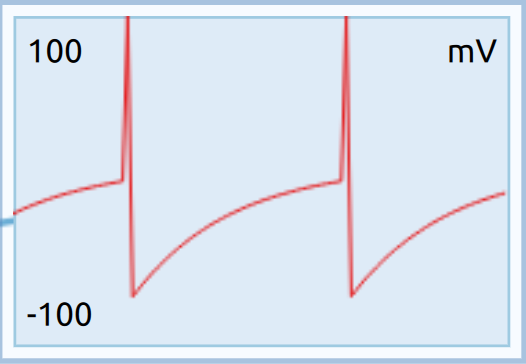
\includegraphics[width = 0.14\paperwidth ]{figures/integrate.png}};
    \node [xshift=-2.cm,yshift=1.5cm, right] at (current page.center)
          { Integrate and fire neurons};
  \end{tikzpicture}

  \begin{tikzpicture}[remember picture,overlay]  
    \node [xshift=-2cm,yshift=-.5cm] at (current page.center)
          {
\includegraphics[width = 0.12\paperwidth ]{figures/logo.png}};
    \node [xshift=1cm,yshift=-.5cm, left] at (current page.center)
          { Neuronify };
  \end{tikzpicture}

  \begin{tikzpicture}[remember picture,overlay]  
    \node [xshift=-.5cm,yshift=-2.5cm] at (current page.center)
          {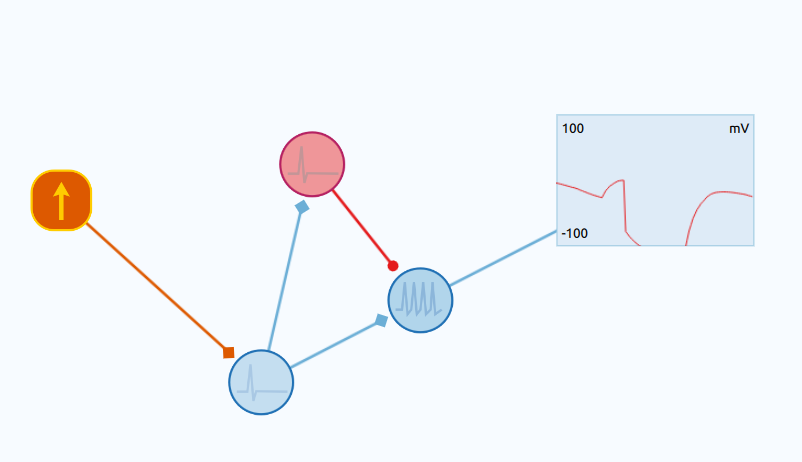
\includegraphics[width = 0.2\paperwidth ]{figures/exercises.png}};
    \node [xshift=2.8cm,yshift=-2.5cm, left] at (current page.center)
          { Exercises};
  \end{tikzpicture}

\end{frame}

\begin{frame}
\frametitle{We do not need all information in the action potential for a neuron in a network and can create an approximation}
\begin{figure}
\includegraphics<1>[width = \textwidth]{figures/hh.png}
\includegraphics<2>[width = 1\textwidth]{figures/fi.png}
\includegraphics<3>[width = 1\textwidth]{figures/fis.png}
\includegraphics<4>[width = 1\textwidth]{figures/all.png}
\end{figure}
\end{frame}


\begin{frame}
\frametitle{The integrate and fire neuron is much faster to evaluate than the Hodgkin-Huxley neuron}

\begin{block}{Hodgkin-Huxley}
\pause
\tiny
\begin{align*}
 C\frac{dV}{dt} &= I_{inj} - \bar{g}_{Na}m^3h(V-V_{Na}) -\bar{g}_Kn^4(V-V_K) - g_L (V-V_L)\\
 \frac{dn}{dt} &= \alpha_n(V) (1-n) - \beta_n(V)n \quad
 \frac{dm}{dt} = \alpha_m(V) (1-m) - \beta_m(V)m\\
 \frac{dh}{dt} &= \alpha_h(V) (1-h) - \beta_h(V)h \quad
 \alpha_n(V) = \frac{0.01(V+55)}{1-\exp[-(V+55)/10]} \\
 \beta_n(V) &= 1.125\exp[-(V+65)/80] \quad
 \alpha_m(V)  = \frac{0.1(V+40)}{1-\exp[-(V+40)/10]} \\
 \beta_m(V) &= 4\exp[-(V+65)/18] \quad
 \alpha_h(V) = 0.07\exp[-(V+65)/20] \\
 \beta_n(V) &= \frac{1}{1+\exp[-(V+35)/10]}
\end{align*}
\end{block}
\pause
\begin{block}{Integrate and fire}
\pause
\tiny
\begin{equation*}
C_m \frac{dV(t)}{dt} = - \frac{V(t) - E_m}{R_m} + I
\end{equation*}
\end{block}
\end{frame}

%\begin{frame}
%\frametitle{Example: learning in mice (Vasilaki et. al., 2009)}
%\begin{figure}
%\includegraphics<1>[width = \textwidth]{figures/morris-watermaze.jpg}
%\includegraphics<2>[width = 1\textwidth]{figures/vasilaki.png}
%\includegraphics<3>[width = 8cm]{figures/vasilaki2.png}
%\end{figure}
%\end{frame}

\begin{frame}
 \frametitle{The integrate and fire model is modeled as a simple RC circuit that is shortcircuted once a threshold is reached}

\begin{figure}
 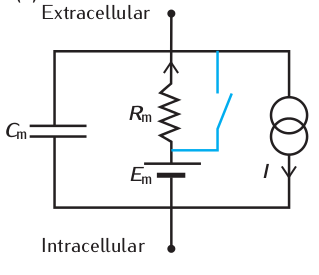
\includegraphics[width = 0.5\textwidth]{figures/rcA.png}
% \includegraphics<2>[width = 0.5\textwidth]{rcAI.png}
% \includegraphics<3>[width = 0.5\textwidth]{rcARm.png}
% \includegraphics<4>[width = 0.5\textwidth]{rcAEm.png}
% \includegraphics<5>[width = 0.5\textwidth]{rcACm.png}
% \includegraphics<6>[width = 0.5\textwidth]{rcAs.png}
% % \includegraphics<7>[width = 0.5\textwidth]{rcB.png}
% % \includegraphics<8>[width = 0.5\textwidth]{rcBs.png}
 \end{figure}
\pause
\begin{equation*}
C_m \frac{dV(t)}{dt} = - \frac{V(t) - E_m}{R_m} + I
\end{equation*}
 \end{frame}

% % % % % % % % % % % % % % % % % % % % % % % % % % % % % % % % % % % % % % % % % %
% Adaptation
% % % % % % % % % % % % % % % % % % % % % % % % % % % % % % % % % % % % % % % % % % %


% % % % % % % % % % % % % % % % % % % % % % % % % % % % % % % % % % % % % % % % % %
% Poisson Generators.
% % % % % % % % % % % % % % % % % % % % % % % % % % % % % % % % % % % % % % % % % % %

% % % % % % % % % % % % % % % % % % % % % % % % % % % % % % % % % % % % % % % % % %
% Receptive Field
% % % % % % % % % % % % % % % % % % % % % % % % % % % % % % % % % % % % % % % % % % %

\begin{frame}
 \frametitle{Receptive Field}


\begin{equation}
r(t) = r_0 + \displaystyle \int \int D(\mathbf{r},\tau) s(\mathbf{r},t-\tau) d\tau d\mathbf{r}
\end{equation}


\begin{figure}
 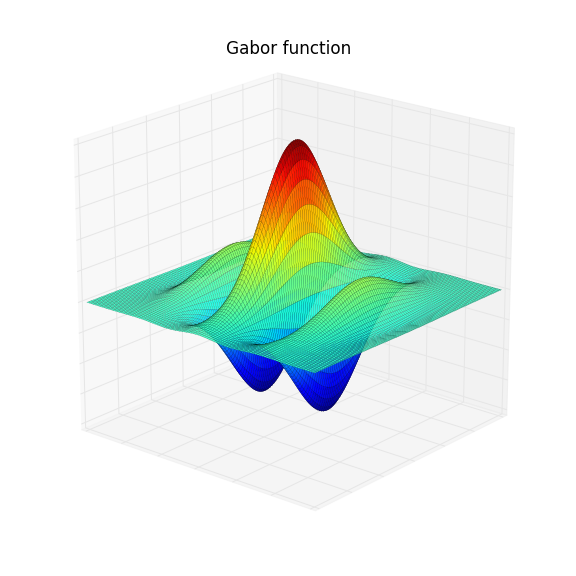
\includegraphics[width = 0.5\textwidth]{figures/gabor.png}
 \end{figure}

\end{frame}


\begin{frame}
 \frametitle{Receptive Field}

\begin{figure}
 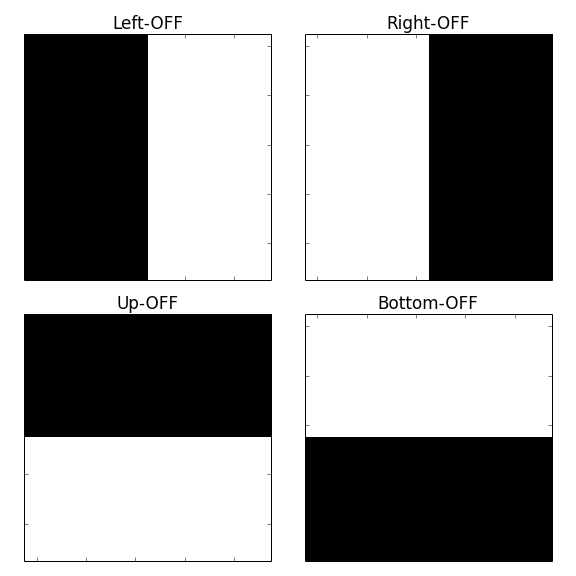
\includegraphics[width = 0.5\textwidth]{figures/recRFs.png}
 \end{figure}

\end{frame}



%
%\begin{frame}
%\frametitle{Neuronify is a new tool for creating neural networks}
%
%
%\begin{figure}
%
\includegraphics[height = 0.6\textheight]{figures/logo.png}
%\end{figure}
%
%\begin{alert}{Download:}\\
%  \scriptsize
%  \href{http://cinpla.org/neuronify/}{http://cinpla.org/neuronify/}
%\end{alert}
%\end{frame}
%
%
%\begin{frame}
%\frametitle{Exercises}
%
%
%\begin{figure}
%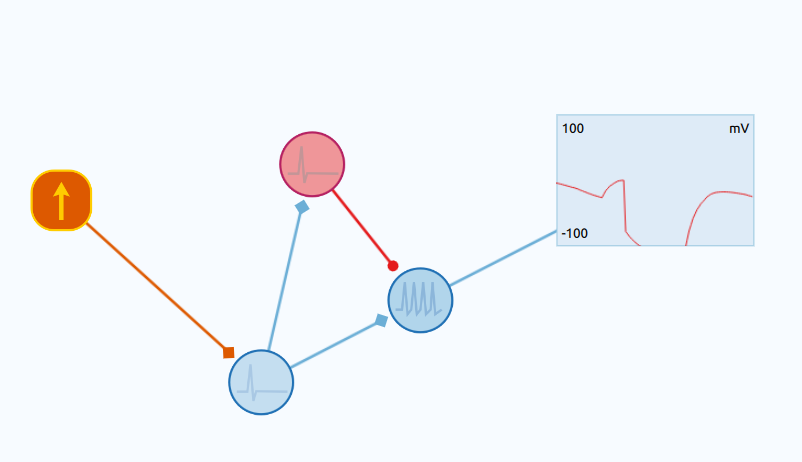
\includegraphics[width = \textwidth]{figures/exercises.png}
%\end{figure}
%\begin{alert}{Exercises:}\\
%  \scriptsize
%  \href{http://cinpla.org/neuronify/}{http://cinpla.org/neuronify/}\\
%\end{alert}
%\end{frame}

\end{document}
